% Options for packages loaded elsewhere
\PassOptionsToPackage{unicode}{hyperref}
\PassOptionsToPackage{hyphens}{url}
%
\documentclass[
]{article}
\usepackage{lmodern}
\usepackage{amssymb,amsmath}
\usepackage{ifxetex,ifluatex}
\ifnum 0\ifxetex 1\fi\ifluatex 1\fi=0 % if pdftex
  \usepackage[T1]{fontenc}
  \usepackage[utf8]{inputenc}
  \usepackage{textcomp} % provide euro and other symbols
\else % if luatex or xetex
  \usepackage{unicode-math}
  \defaultfontfeatures{Scale=MatchLowercase}
  \defaultfontfeatures[\rmfamily]{Ligatures=TeX,Scale=1}
\fi
% Use upquote if available, for straight quotes in verbatim environments
\IfFileExists{upquote.sty}{\usepackage{upquote}}{}
\IfFileExists{microtype.sty}{% use microtype if available
  \usepackage[]{microtype}
  \UseMicrotypeSet[protrusion]{basicmath} % disable protrusion for tt fonts
}{}
\makeatletter
\@ifundefined{KOMAClassName}{% if non-KOMA class
  \IfFileExists{parskip.sty}{%
    \usepackage{parskip}
  }{% else
    \setlength{\parindent}{0pt}
    \setlength{\parskip}{6pt plus 2pt minus 1pt}}
}{% if KOMA class
  \KOMAoptions{parskip=half}}
\makeatother
\usepackage{xcolor}
\IfFileExists{xurl.sty}{\usepackage{xurl}}{} % add URL line breaks if available
\IfFileExists{bookmark.sty}{\usepackage{bookmark}}{\usepackage{hyperref}}
\hypersetup{
  pdftitle={Improving the IEA approach using principles of open data science},
  pdfauthor={Kimberly Bastille1; Sean Hardison2; Lynn DeWitt3; Jennifer Brown4; Jameal Samhouri5; Sarah Gaichas6; Sean Lucey6; Kelly Kearney7; Ben Best8; Scott Cross9; Scott Large6; Ellen Spooner10},
  hidelinks,
  pdfcreator={LaTeX via pandoc}}
\urlstyle{same} % disable monospaced font for URLs
\setlength{\emergencystretch}{3em} % prevent overfull lines
\providecommand{\tightlist}{%
  \setlength{\itemsep}{0pt}\setlength{\parskip}{0pt}}
\setcounter{secnumdepth}{-\maxdimen} % remove section numbering
\usepackage{graphicx}
\usepackage{array}
\usepackage{booktabs}
\usepackage{multirow}
\usepackage{subfig}
\usepackage{longtable}
\usepackage{wrapfig}
\usepackage{float}
\usepackage{colortbl}
\usepackage{pdflscape}
\usepackage{tabu}
\usepackage{threeparttable}
\usepackage{threeparttablex}
\usepackage[normalem]{ulem}
\usepackage{makecell}
\usepackage{xcolor}

\usepackage[export]{adjustbox}
\newlength{\cslhangindent}
\setlength{\cslhangindent}{1.5em}
\newenvironment{cslreferences}%
  {\setlength{\parindent}{0pt}%
  \everypar{\setlength{\hangindent}{\cslhangindent}}\ignorespaces}%
  {\par}

\title{Improving the IEA approach using principles of open data science}
\author{Kimberly Bastille\textsuperscript{1} \and Sean
Hardison\textsuperscript{2} \and Lynn
DeWitt\textsuperscript{3} \and Jennifer
Brown\textsuperscript{4} \and Jameal
Samhouri\textsuperscript{5} \and Sarah
Gaichas\textsuperscript{6} \and Sean Lucey\textsuperscript{6} \and Kelly
Kearney\textsuperscript{7} \and Ben Best\textsuperscript{8} \and Scott
Cross\textsuperscript{9} \and Scott Large\textsuperscript{6} \and Ellen
Spooner\textsuperscript{10}}
\date{}

\begin{document}
\maketitle
\begin{abstract}
The text of your abstract. 150 -- 250 words.
\end{abstract}

\textsuperscript{1} Integrated Statistics, Woods Hole, MA, USA\\
\textsuperscript{2} University of Virginia, Charlottesville, VA, USA\\
\textsuperscript{3} Three\\
\textsuperscript{4} Four\\
\textsuperscript{5} Five\\
\textsuperscript{6} Woods Hole Laboratory, NOAA NMFS Northeast Fisheries
Science Center, Woods Hole, MA, USA\\
\textsuperscript{7} University of Washington, Joint Institute for the
Study of the Atmosphere and Ocean, Seattle, WA, USA\\
\textsuperscript{8} EcoQuants LLC, Santa Barbara, CA, USA\\
\textsuperscript{9} nine\\
\textsuperscript{10} ten

\hypertarget{intro}{%
\section{Introduction}\label{intro}}

As implemented so far, integrated ecosystem assessments are more often
than not bespoke products that are specific to regional policy needs at
varying spatial scales. While unique, these assessments are typically
built around the flow of the IEA framework outlined in (Levin et al.
2009). This process consists of a scoping step to outline management
objectives, the identification of ecosystem indicators to monitor key
processes, the compilation of ecosystem status reports highlighting
status and trends of indicators, a risk assessment step identifying
where ecosystem considerations might threaten management objectives, and
finally management strategy evaluation, in which potential management
actions are tested using simulation models. The elements of the IEA
framework are central to its implementation, but its flow is not
prescriptive. Instead, the IEA process is malleable to the needs of
stakeholders, meaning that IEAs may manifest in many different forms.

However, data acquisition, management, communication, and dissemination
are universal challenges that apply across the disparate applications of
IEAs. Solving these challenges is not trivial, but over the past decade
several examples have emerged suggesting the use of open data science
tools as potential solutions (Rocchini and Neteler 2012; Lowndes et al.
2015; Lowndes et al. 2017; Ma et al. 2018). For example, Lowndes et
al.~2017 discussed how embracing open science methods allowed for
increased efficiency, transparency, and reproducibility in the
development of the Ocean Health Index; a modular framework developed to
assess the benefits of marine ecosystems to humans for sustainable
management. Case studies for applying open science processes to IEAs
have also been developed for ecosystem reporting in the Northeast Large
Marine Ecosystem. Specifically, Ma et al.~2017 show how machine-readable
provenance may be incorporated into automated analytical workflows using
IPython and the Semantic Web.

Embracing these tools and strategies speaks to a broader philosophy of
open science that has yet to fully catch on in the IEA community. Beyond
making data publicly available, open science advocates for the ``free
and unfettered access to all aspects of the scientific endeavor''
(Hampton et al. 2015), including methods, data and scientific products.
These values lend themselves to the broad applicability of IEAs as
decision-making tools for ecosystem-based management (EBM).

There are several entry and exit points for data, methodological, and
scientific products throughout the execution of an IEA. Data entry
points are formed during the exploratory phases of the IEA process,
where objectives are scoped and representative indicators are developed.
Exit points for data products can be found in the derived indicator data
informing ecosystem status reports and risk assessments. Simulated
products and model parameters, such as those resulting from MSE model
runs, are also important to disseminate. Any data that leaves or enters
an IEA brings with it metadata and code used to analyze, process, and
visualize the data (in various stages of completion). Through the
process these datasets, accompanying code, and metadata documentation
become their own general, scientific and technical products feeding into
subsequent products and adding transparency and efficiency (Fig.
@ref(fig:iealoop)).

Without an underlying data management protocol, the vast quantities of
data and documentation required to successfully execute an IEA can be
overwhelming for practitioners and clients both. For example, the
development of ecosystem status reports and risk assessments requires
considering the management relevance of hundreds of data sets from many
fields. In practice this meant sifting through over 400 unique spatial
and temporal data sets that were submitted for consideration during the
development of the New England State of the Ecosystem Report, an IEA
product. However, only indicators of interest to managers and those
necessary for storytelling were included in the final product; just over
90 (Gaichas, Sarah and Hardison, Sean and Large, Scott and Lucey, Sean
2019). Depending on the governing body implementing the IEA, each data
set must be fully documented with metadata and made publicly available.
Versioning data sets and associated metadata relative to specific IEA
products also introduces challenges for scientists operating outside the
bounds of their training. These hurdles result in data processing and
documentation becoming a full time job, and indeed, it is becoming
increasingly common for IEA teams to hire Data Analysts and Data
Scientists to deal with the data deluge.

\begin{figure}
  \centering
  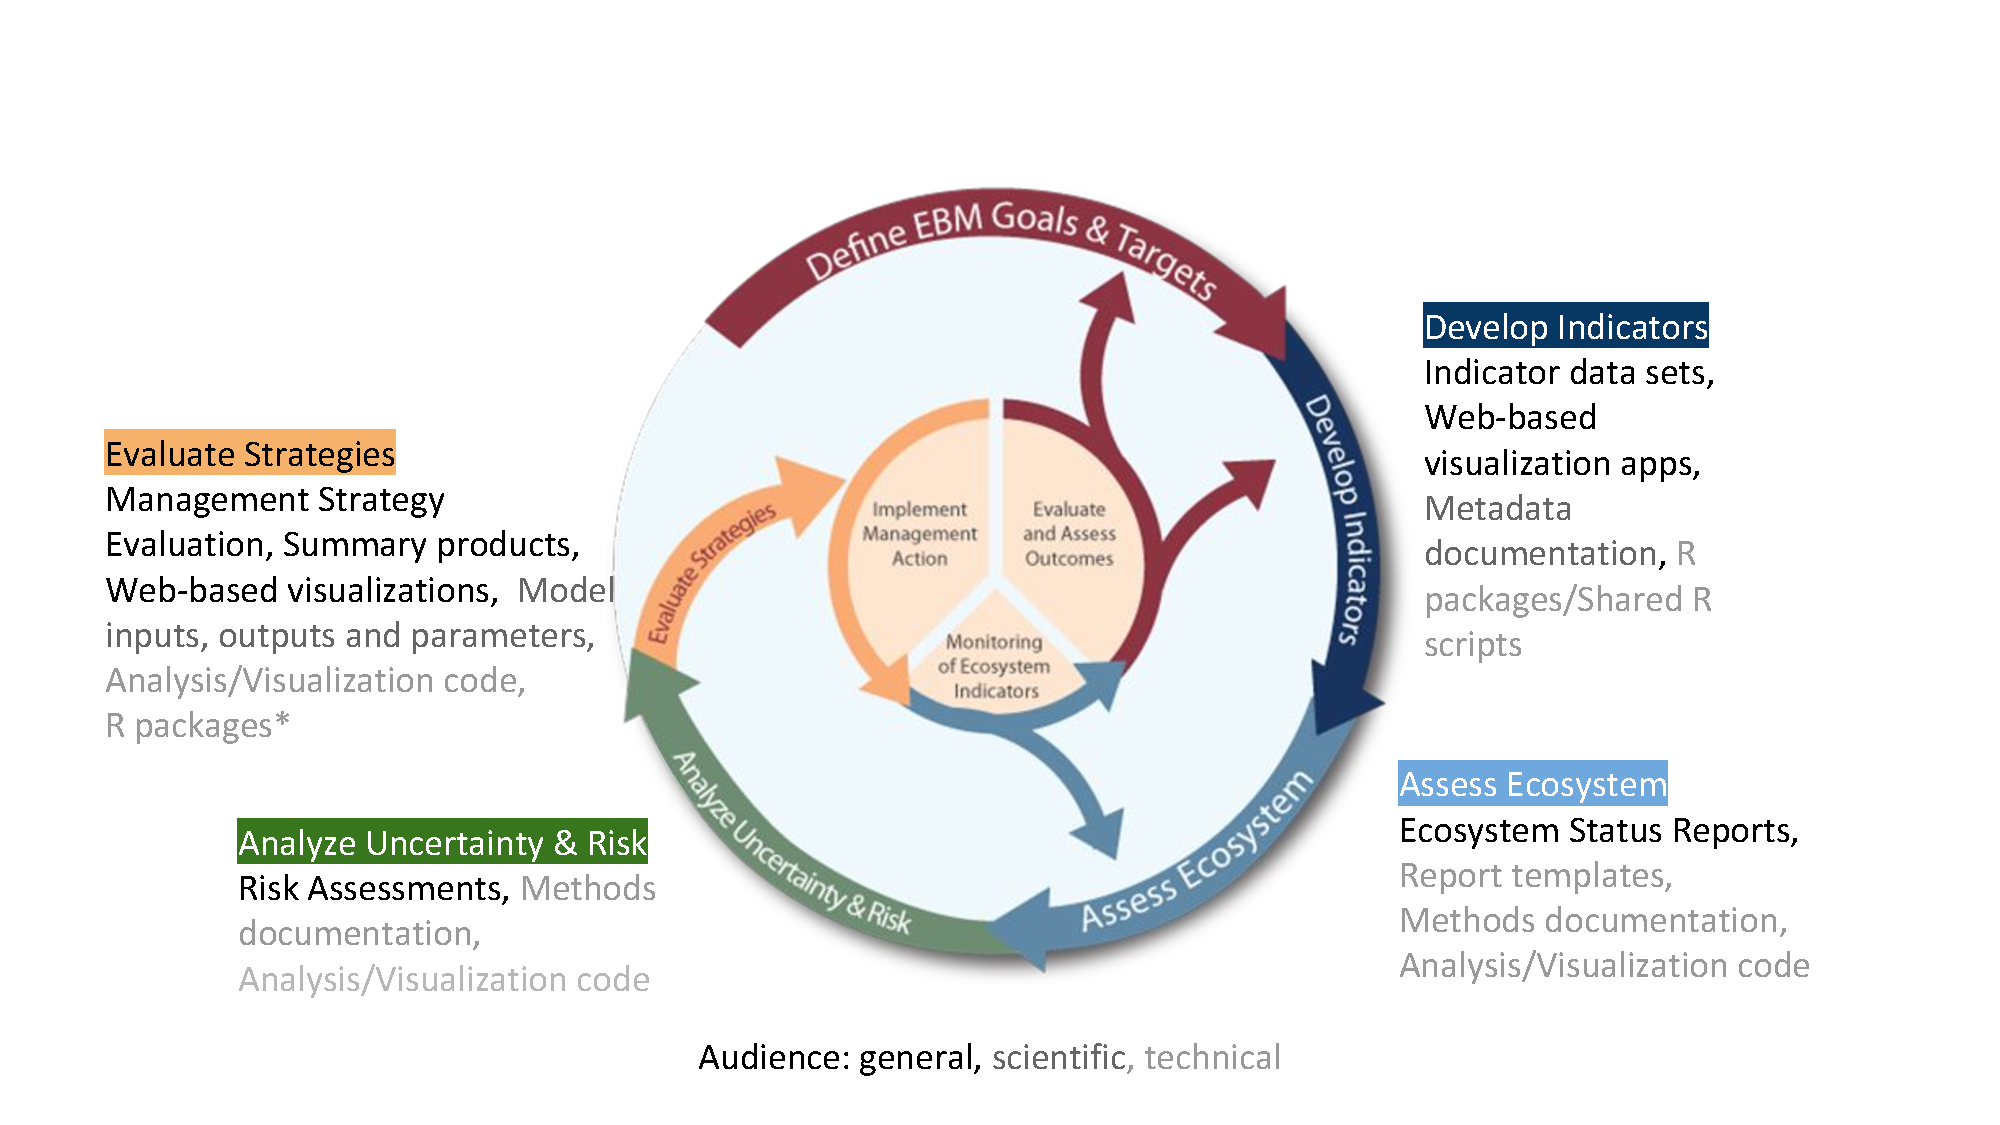
\includegraphics[width=1.0\textwidth]{./images/products-loop.pdf}
  \caption{Products as part of the IEA loop according to audience: general, scientific and technical.}
  \label{fig:products-loop}
\end{figure}

The implementation of IEA is an amalgam of the ecosystem and data
sciences. Understanding this, we suggest that IEA teams embrace a
philosophy of open science. This approach has gained momentum over the
past decade within the ecological sciences as a way to deal with large
amounts of data produced from a variety of sources (Michener and Jones
2012), as well as to improve transparency, reproducibility,
repeatability, and ease of communication of data products (Rocchini and
Neteler 2012; Lowndes et al. 2015; Lowndes et al. 2017; Ma et al. 2018).
This can be accomplished using openly available tools, many of which are
highlighted by Hampton et al. (2015) and Lowndes et al. (2017).

The benefits of implementing software development strategies range from
the ethical to the practical. For example, Lowndes et al. (2017)
suggests that changing ecosystem conditions due to anthropogenic impacts
necessitate openness among environmental scientists whose data (and code
to recreate their data) provide ``snapshots'' of their study systems
amidst the changes. Further, openly-sourcing scientific data with
accompanying code provides a record from which previous results may be
built upon as more data are collected (Lowndes et al. 2017). From this
perspective, iterative IEA products such as ecosystem reports and risk
assessments are themselves data points; forming ever-extending arrays of
compiled information through time. This approach has been embraced by
the Ocean Health Index, which is designed to monitor human-ocean
relationships through time by repeated compilation and analysis of
ecosystem data (Halpern et al. 2012; Halpern et al. 2015; Lowndes et al.
2015).

We suggest that the incorporation of version control and standardized
methods for the collection, aggregation, and dissemination of
IEA-oriented data and products can facilitate flexible and efficient use
of IEAs, broadening their applicability and hastening their uptake by
resource managers. These methods also confront the challenging spatial
aspects of IEAs, which are inherently unique to the systems being
addressed. As we discuss below, embracing standardized methods and open
data science principles/tools would facilitate the implementation of
future IEAs in new systems.

\begin{figure}
  \centering
  \subfloat[Process]{           
    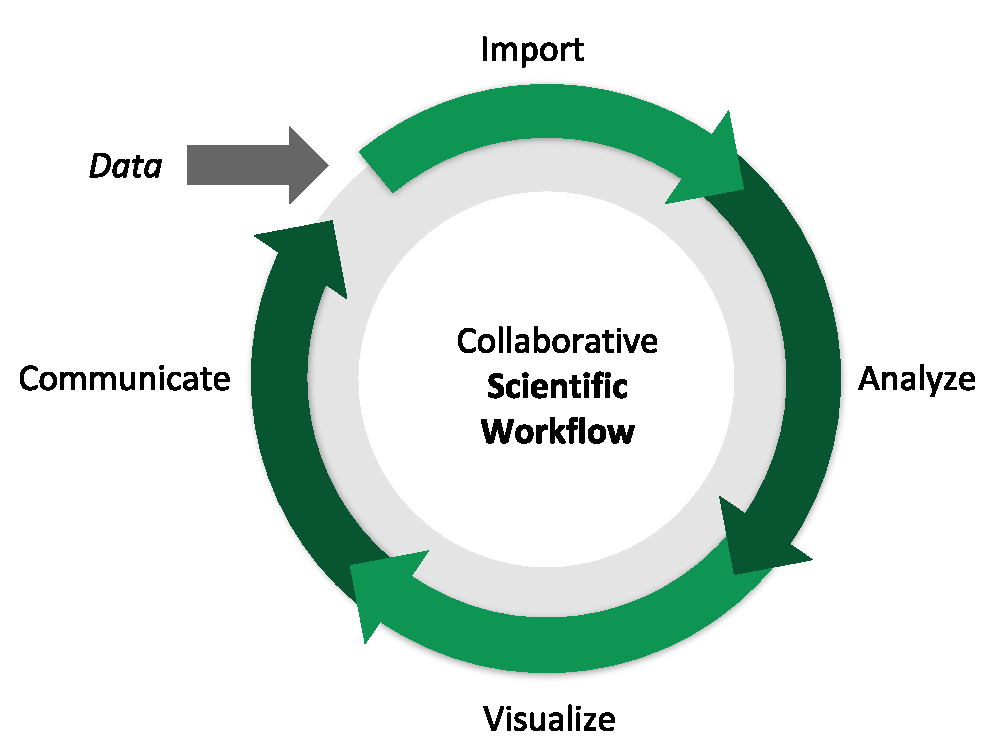
\includegraphics[width=0.50\textwidth,valign=t]{./images/sciloop.pdf}
    \label{fig:sciflow-loop}
    }
  \subfloat[Elements]{
    \adjustbox{valign=t}{
      \begingroup\fontsize{5}{7}\selectfont
\begin{tabular}{>{\bfseries}l>{\raggedright\arraybackslash}p{10em}l}
\toprule
Function & Implementation & Tool\\
\midrule
 & ecodata & R package\\
\cmidrule{2-3}
\multirow{-2}{*}{\raggedright\arraybackslash Import} & Data portals & ERDDAP\\
\cmidrule{1-3}
 & lm to ecosystem modelling & Shared R scripts\\
\cmidrule{2-3}
 & ecotrend & R package\\
\cmidrule{2-3}
\multirow{-3}{*}{\raggedright\arraybackslash Analyze} & Ecosystem modelling & Ecopath with Ecosim\\
\cmidrule{1-3}
 & Standardized plotting & Shared R scripts\\
\cmidrule{2-3}
 & Web-based visuals & Shiny\\
\cmidrule{2-3}
\multirow{-3}{*}{\raggedright\arraybackslash Visualize} & Simple plots & Excel\\
\cmidrule{1-3}
 & Report writing, article writing, methods documentation & Rmarkdown\\
\cmidrule{2-3}
 & Continuous integration & Travis\\
\cmidrule{2-3}
 & Versioning software & Git\\
\cmidrule{2-3}
 & Collaborative package/document development and data sharing & Github\\
\cmidrule{2-3}
\multirow{-5}{*}{\raggedright\arraybackslash Communicate} & Data portals & ERDDAP\\
\bottomrule
\end{tabular}
\endgroup{}

      \label{tbl:sciflow-table}}}
  \caption{Scientific workflow.}
\end{figure}

\hypertarget{references}{%
\section{References}\label{references}}

\hypertarget{refs}{}
\begin{cslreferences}
\leavevmode\hypertarget{ref-SOE-NEFMC2019}{}%
Gaichas, Sarah and Hardison, Sean and Large, Scott and Lucey, Sean.
2019. State of the ecosystem 2019: New england. 166 Water Street, Woods
Hole, MA 02543-1026: National Marine Fisheries Service, NEFSC.

\leavevmode\hypertarget{ref-halpern2012}{}%
Halpern, Benjamin S., Catherine Longo, Darren Hardy, Karen L. McLeod,
Jameal F. Samhouri, Steven K. Katona, Kristin Kleisner, et al. 2012. An
index to assess the health and benefits of the global ocean.
\emph{Nature}. \url{https://doi.org/10.1038/nature11397}.

\leavevmode\hypertarget{ref-halpern2015}{}%
Halpern, Benjamin S., Catherine Longo, Julia S. Stewart Lowndes,
Benjamin D. Best, Melanie Frazier, Steven K. Katona, Kristin M.
Kleisner, Andrew A. Rosenberg, Courtney Scarborough, and Elizabeth R.
Selig. 2015. Patterns and Emerging Trends in Global Ocean Health.
\emph{PLoS ONE} 10: e0117863.
\url{https://doi.org/10.1371/journal.pone.0117863}.

\leavevmode\hypertarget{ref-hampton2015}{}%
Hampton, Stephanie E, Sean S Anderson, Sarah C Bagby, Corinna Gries,
Xueying Han, Edmund M Hart, Matthew B Jones, et al. 2015. The tao of
open science for ecology. \emph{Ecosphere} 6. Wiley Online Library:
1--13.

\leavevmode\hypertarget{ref-Levin2009}{}%
Levin, Phillip S, Michael J Fogarty, Steven A Murawski, and David
Fluharty. 2009. Integrated ecosystem assessments: Developing the
scientific basis for ecosystem-based management of the ocean. \emph{PLOS
Biology} 7. Public Library of Science: 1--6.
\url{https://doi.org/10.1371/journal.pbio.1000014}.

\leavevmode\hypertarget{ref-lowndes2017}{}%
Lowndes, Julia S Stewart, Benjamin D Best, Courtney Scarborough, Jamie C
Afflerbach, Melanie R Frazier, Casey C O'Hara, Ning Jiang, and Benjamin
S Halpern. 2017. Our path to better science in less time using open data
science tools. \emph{Nature ecology \& evolution} 1. Nature Publishing
Group: 0160.

\leavevmode\hypertarget{ref-lowndes2015}{}%
Lowndes, Julia S Stewart, Erich J Pacheco, Benjamin D Best, Courtney
Scarborough, Catherine Longo, Steven K Katona, and Benjamin S Halpern.
2015. Best practices for assessing ocean health in multiple contexts
using tailorable frameworks. \emph{PeerJ} 3. PeerJ Inc.: e1503.

\leavevmode\hypertarget{ref-ma2018}{}%
Ma, Xiaogang, Stace E Beaulieu, Linyun Fu, Peter Fox, Massimo Di
Stefano, and Patrick West. 2018. Documenting provenance for reproducible
marine ecosystem assessment in open science. In \emph{Information
retrieval and management: Concepts, methodologies, tools, and
applications}, 1051--1077. IGI Global.

\leavevmode\hypertarget{ref-michener2012}{}%
Michener, William K, and Matthew B Jones. 2012. Ecoinformatics:
Supporting ecology as a data-intensive science. \emph{Trends in ecology
\& evolution} 27. Elsevier: 85--93.

\leavevmode\hypertarget{ref-rocchini2012}{}%
Rocchini, Duccio, and Markus Neteler. 2012. Let the four freedoms
paradigm apply to ecology. \emph{Trends in ecology \& evolution} 27.
Elsevier: 310--311.
\end{cslreferences}

\end{document}
